\section{Introduction}

Bitcoin~\cite{nakamoto2008bitcoin} is the most popular cryptocurrency, and, while volatile, has a market cap consistently over half a trillion dollars since January of 2021.   Bitcoin Core (\url{https://github.com/Bitcoin/Bitcoin}) is by far the most popular implementation, and serves as a reference for all other implementations of Bitcoin.  To a significant degree, the code of Bitcoin Core \emph{is} Bitcoin.  Because of its fame and the high value of Bitcoins, Bitcoin is a high-value target for hackers.  Therefore, testing the code is of paramount importance, including extensive functional tests and aggressive \emph{fuzzing}.  This paper describes a focused effort to identify weaknesses in, and improve, the fuzzing of Bitcoin Core.

%\section{Initial Contact and the Problem of Saturation}

Chaincode Labs (\url{https://chaincode.com/}) is a private R\&D center that exists solely to support and develop Bitcoin.  In March of 2021 the head of special projects at Chaincode contacted the first author to discuss determining a strategy to improve the fuzzing of Bitcoin Core.  It seemed that the fuzzing was ``stuck'': neither code coverage nor found bugs were increasing with additional fuzzing.  After some discussion, an 80 hour effort was determined as a reasonable scope for an external, research-oriented, look at the fuzzing effort.

%Before that effort, conducted over the summer of 2021, began, the problem of saturation resolved itself.  Nonetheless, the issue that drove the initial %desire for a researcher investigation is well worth examining.  Moreover, understanding why Bitcoin Core fuzzing was, temporarily but not %fundamentally, saturated, may be useful to help other fuzzing campaigns avoid the same false saturation problem.

Saturation, as defined in the blog post (\url{https://blog.regehr.org/archives/1796}) that brought Chaincode Labs to the first author, is when ``We apply a fuzzer to some non-trivial system... [and] the number of new bugs found by the fuzzer drops off, eventually approaching zero.''  At first a particular fuzzer applied to a system will tend to continuously increase both coverage and discovery of previously-unknown bugs.  But, at some point, these bugs are known (and often fixed) and the fuzzer stops producing new bugs.  Code and behavioral coverage seems to be \emph{saturated}.
The underlying reason for saturation is that any fuzzer (or other test generator) explores a space of generated tests according to some complex probability distribution.  Some bugs lie in the high-probability portion of this space, and other bugs lie in very low probability zero probability parts.  Escaping saturation may require a variety of approaches.

\section{Results}

One thing that quickly emerged from discussions before the primary 80 hour effort began was the limited extent of the fuzzer runs being performed.  The fuzzing includes a large number of targets, each with its own fuzz harness and executable.  At the time, the basic strategy was to run libFuzzer on each of these for 100,000 iterations.  Because some targets are very fast and a few, such as full message processing, are slow, this meant in practice fuzzing most targets for only 30-90 seconds, and even the slowest targets for only a little over an hour.  The total time for over 100 targets was not negligible, but expecting such short runs for each target, after an initial exploration of the easy part of the probability space, to gain coverage or bugs very often, was simply unrealistic.  For complex targets such as transaction verification and end-to-end message processing, 100,000 iterations was highly insufficient.   The first suggestion for escaping saturation, therefore was very simple:  run the fuzzer longer!  The Chaincode tried increasing their configuration to 5 million iterations, multiplying the number of executions by a factor of 50.  Based on initial success with a few targets, this was done for all targets, and became the new default.  By May 20th, Bitcoin Core was also in OSS-Fuzz: \url{https://github.com/google/oss-fuzz/tree/master/projects/bitcoin-core}.  From then on, Bitcoin Core has essentially been continuously fuzzed, and OSS-Fuzz quickly produced new crashes to investigate, and continues to do so:  \url{https://bugs.chromium.org/p/oss-fuzz/issues/list?q=bitcoin}.

Additonal efforts to improve the fuzzing focused on adding support for the Eclipser fuzzer~\cite{Eclipser}, and attempting to use swarm testing~\cite{ISSTA12} to produce more unusual message sequence interactions.  Using Eclipser produced a large number of additional corpus seeds for OSS-Fuzz (over 2,000 inputs, the third largest contribution to the set to date), while swarm turned out to be ineffective, due to extensive manual cross-seeding providing similar benefits.  Neither approach, however, turned up any new bugs and improvements were in some sense marginal (new paths or data values only).

\section{Mutation Analysis}

\lstset{style=langstyle}
%\section{Mutation Analysis}

Attempting to improve a fuzzing effort is one way to find problems
with the effort; if you succeed, you found a weakness.  However, none
of the attempts exposed a serious problem.  An alternative is
to directly look for holes in testing.  The Bitcoin Core fuzzing team
clearly was measuring and inspecting code coverage (see \url{https://marcofalke.github.io/btc_cov/}), so little value
would be added by inspecting traditional coverage alone.  Mutation
testing/analysis~\cite{MutationSurvey}, however, subsumes code coverage and adds extremely
valuable information on \emph{oracle power} in addition to mere
coverage~\cite{Discontents}.    In previous work, we had
used mutation testing to improve the random testing of the Linux
kernel's RCU module, and in the process discovered some subtle kernel bugs~\cite{mutKernel,groce2018verified}.

\begin{sloppypar}
We used the Universal Mutator
\noindent(\url{https://github.com/agroce/universalmutator})~\cite{regexpMut} to
mutate transaction
verification code  in the
{\tt tx\_verify.cpp} file; this is clearly extremely critical functionality.  Fuzzing covers 96 of 98 lines of code, 8
of 8 functions, and 74 of 102 branches for this file, guaranteeing
that mutation testing will not primarily reflect missing coverage.
Comparing coverage to that for functional testing, the fuzz testing
has very slightly lower branch coverage, but the numbers are almost
identical (72.5\% vs. 73\%), and the fuzz testing covers \emph{different} branches.  

\begin{figure}
\vspace{2mm}
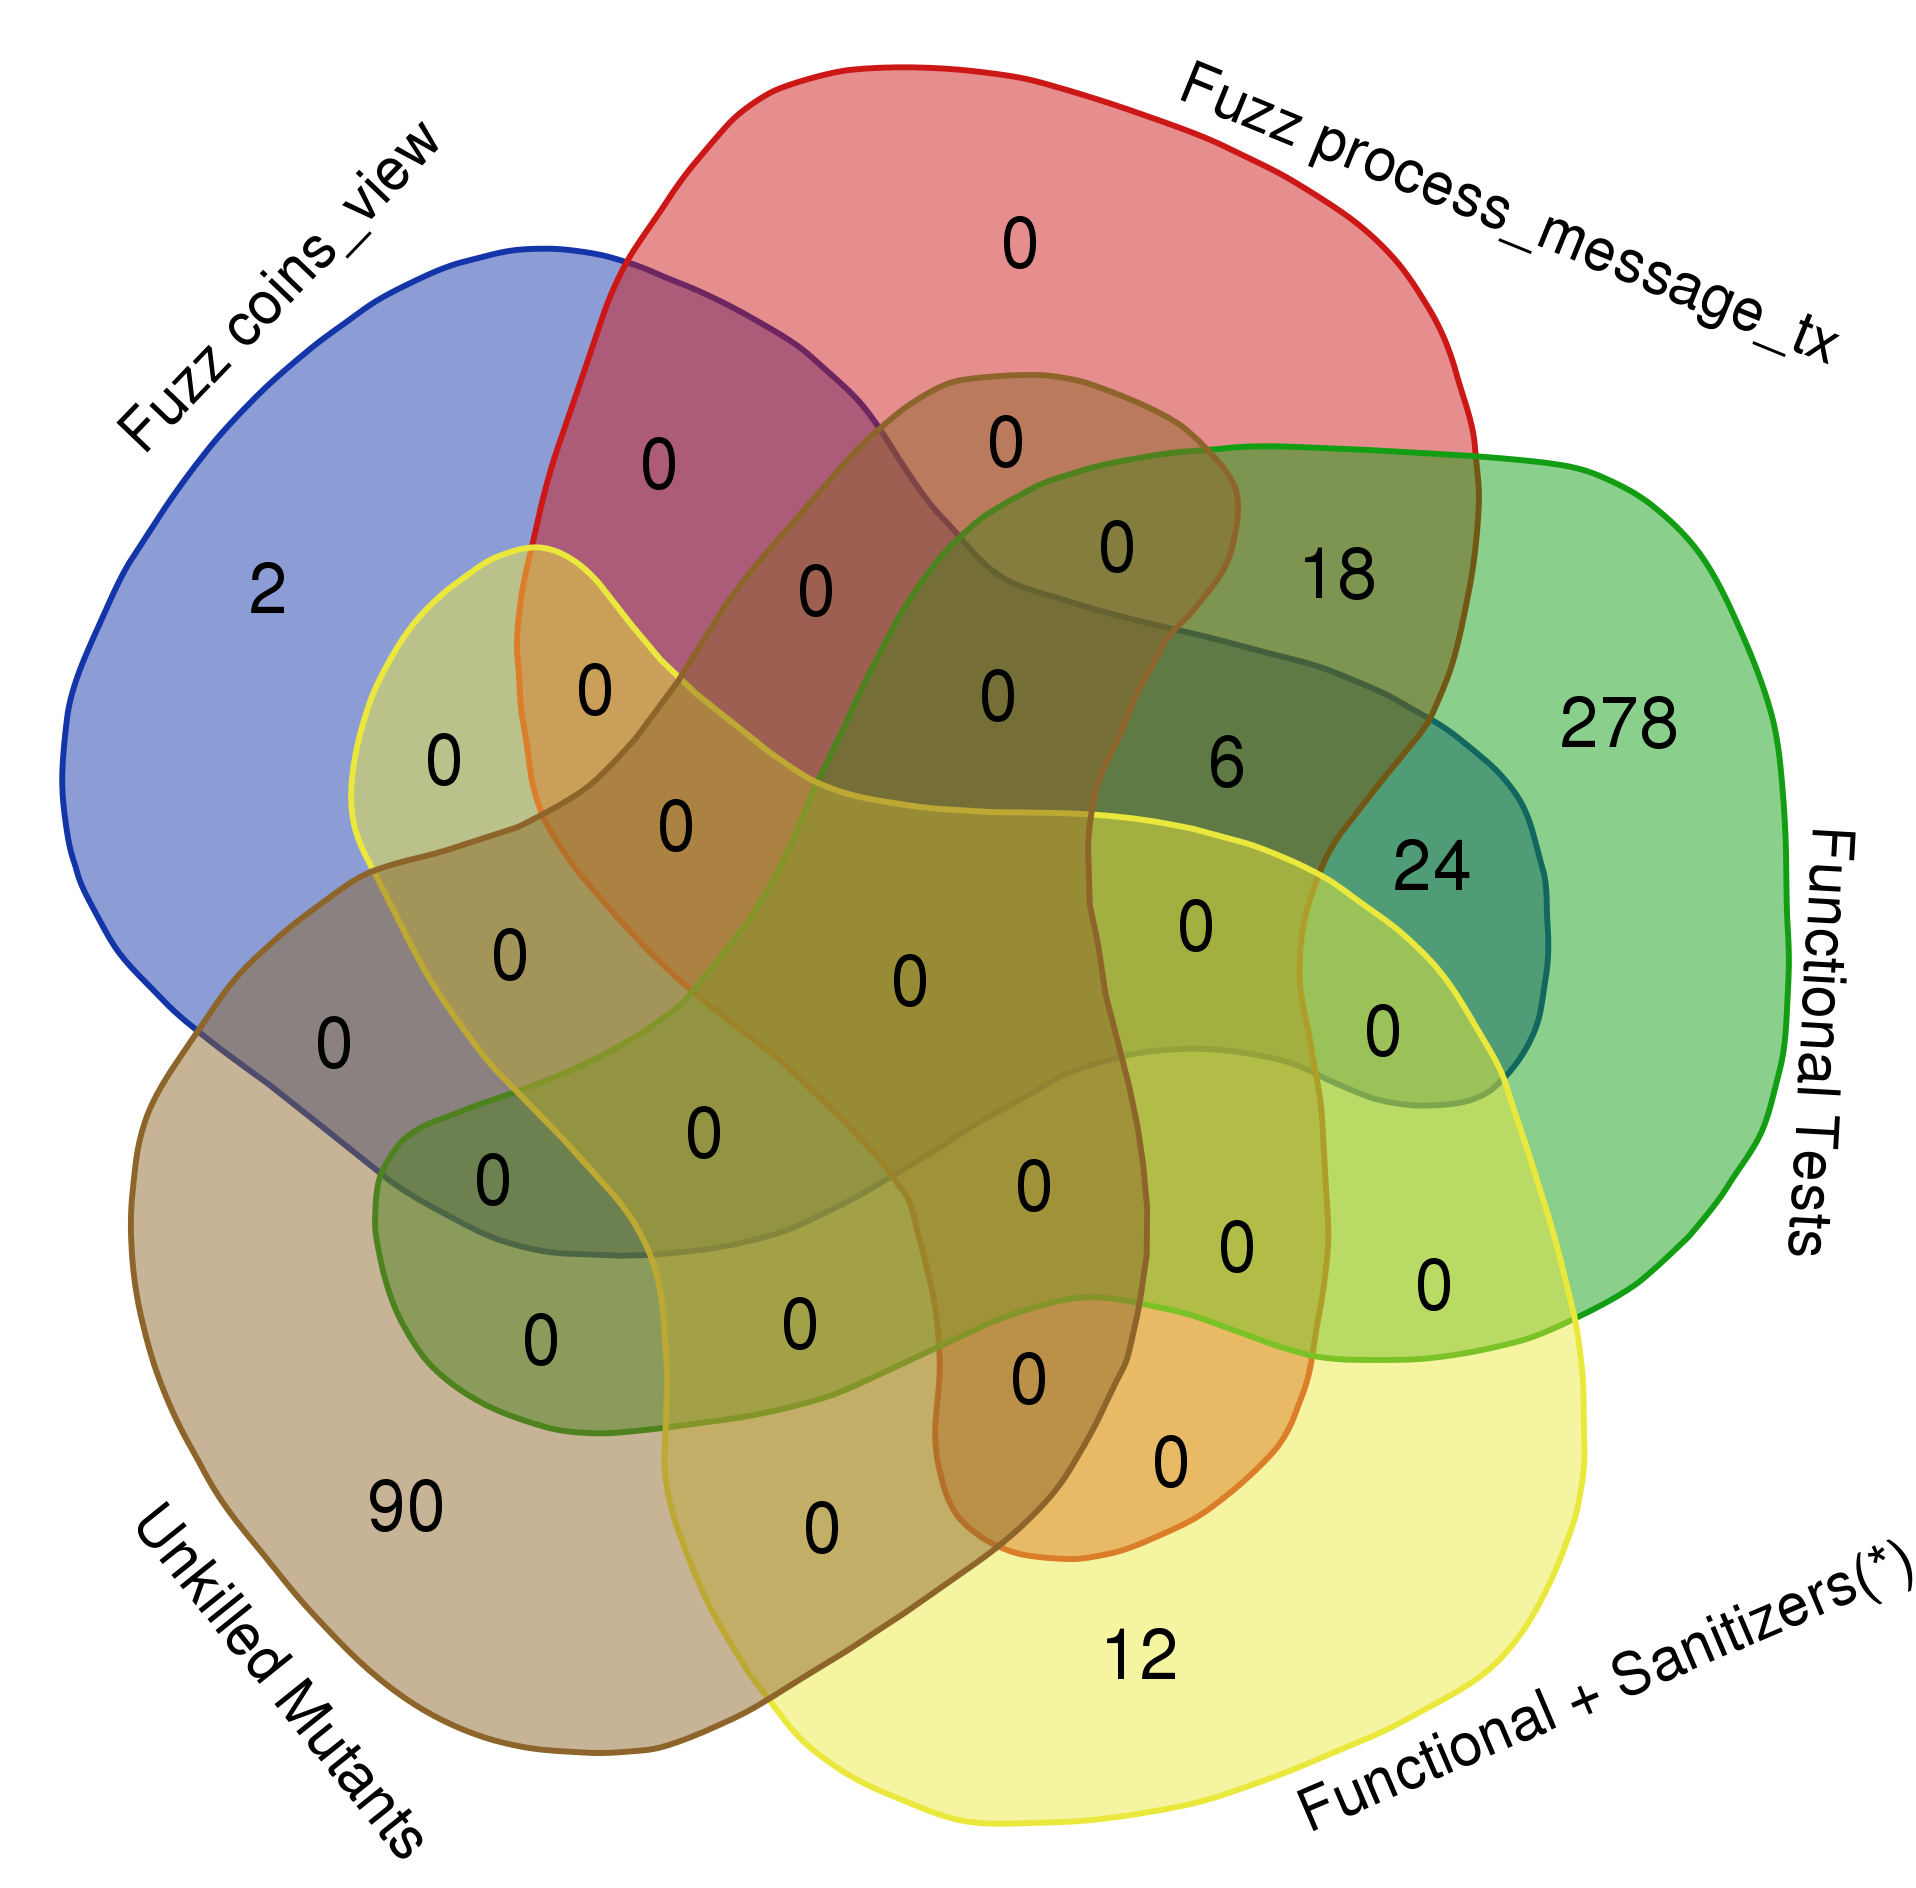
\includegraphics[width=0.6\columnwidth]{kill_pre_valgrind.png}
\caption{Mutation kills for {\tt tx\_verify.cpp}}
\label{kills}
\end{figure}


%{\bf Mutant \#379} changes the {\tt strprintf} to:

%\begin{code}
%strprintf("tried to spend coinbase at depth \%d", nSpendHeight / coin.nHeight));
%\end{code}

%{\bf Mutant \#380} changes the {\tt strprintf} to:

%\begin{code}
%strprintf("tried to spend coinbase at depth \%d", nSpendHeight \% coin.nHeight));
%\end{code}
%}
%\caption{Mutants detected \emph{only} by fuzzing.}
%\label{mkills}
%\end{figure*}

The Universal Mutator generated 430 mutants. The {\tt process\_message\_tx} fuzz target was
able to detect 24 mutants, and the {\tt coins\_view} harness was able to detect
32 mutants, for a total of 50 mutants (since some mutants were
detected by both). Fuzzing could detect just under 12\%
of mutants.   Fuzzing adds only two unique mutant kills beyond those produced by
functional testing, which has a much higher score.  This raises the question:  why fuzz?  
The answer lies in the fact that, even in the presence of such high quality tests, fuzzing
uncovers subtle bugs that functional tests designed by humans will
almost never detect, e.g. \url{https://github.com/bitcoin/bitcoin/issues/22450}.

To put Bitcoin Core in context, we performed mutation analysis
of transaction-verification-related code for other cryptocurrencies, and Bitcoin ranked high: 2nd out of 6 projects. Bitcoin Core
also had the highest File and Project coverage of any project.  

Our conclusion, based on the negligible gap between code coverage for fuzzing and functional tests, and the huge difference in mutation scores, and the lack of new bugs found even when we ran novel fuzzers, is that the best way for Bitcoin to gain fuzzing power might be to improve the oracle power in fuzzing by adding more invariants and sanity checks.  The Bitcoin Core code has about 1,800 {\tt assert}
statements, scattered among  ~180KLOC of C and C++.  The resulting ratio
of about one assertion per 100 lines of code is not terrible, but is
at the lower limit of what many consider to be an acceptable assertion
ratio for critical code.
Given that Bitcoin Core defines at least 4,000 functions, the code obviously
doesn't meet the NASA/JPL proposal of having an average of two
assertions per function~\cite{holzmann2006power}.  There are only five assert
statements in the {\tt src/consensus} directory, which has about 500
lines of code and defines more than 10 functions, suggesting that the assertion ratio is low even for very
critical code.

%\section{Full Report}

{\bf {Full Report:}} The full report on this effort is available at \url{https://agroce.github.io/bitcoin_report.pdf}.
